\documentclass[11pt]{article}
\pdfinfoomitdate=1\pdftrailerid{}\pdfsuppressptexinfo=15
\usepackage[letterpaper,margin=.7in,headheight=15pt,headsep=18pt,footskip=24pt]{geometry}
\usepackage[T1]{fontenc}
\usepackage{lmodern,amsmath,amssymb,array,booktabs,fancyhdr,tikz}
\usetikzlibrary{arrows.meta}
\renewcommand{\familydefault}{\sfdefault}
\setlength{\parindent}{0pt}\setlength{\parskip}{6pt}
\pagestyle{fancy}\fancyhf{}
\renewcommand{\headrulewidth}{0pt}
\fancyhead[L]{\small Week 91 / Rotor-router machines / K--1 adult guide}
\fancyfoot[L]{\scriptsize Bellingham Math Circle / Week 91 / F91-K-FAC-v1}
\fancyfoot[R]{\thepage}
\newcommand{\head}[1]{\par\textbf{\large #1}\par}
\newcommand{\sub}[1]{\par\textbf{#1}\par}
\newcommand{\code}[1]{\texttt{#1}}
\begin{document}
\head{Mathematical overview: taking turns is not tossing a coin}
\textbf{One switch alternates.} Follow the visible arrow, then flip that card; do not reset it between counters. Every pair of consecutive departures sends one counter each way. The exit piles are therefore equal or differ by one, and two consecutive counters never share an exit. Children can explain this by showing the changed arrow and pairing arrivals, without using odd/even vocabulary.

\textbf{The four-exit tree repeats after four counters.} Its top card sends two counters to each lower card; each lower card sends one to each exit. Every card flips an even number of times and returns to its start. Thus successive blocks of four reach A, B, C and D once, in the same order; eight give two each and twelve give three each. This needs the printed equal-depth tree, one counter finishing before the next starts, and no manual card changes within a trial. It is not a claim about arbitrary trees or roads.

\textbf{The start controls order, not just totals.} The three cards have eight possible starts, giving eight different four-arrival orders. The first two counters always enter opposite halves. A route to one chosen exit fixes only the two cards it touches; the unused lower card is free. A coin, by contrast, can choose either exit anew: repeated exits and unequal piles are possible. Fair, independent tosses are assumed only for the probability notes below.

\textbf{Destination and evidence.} K--1 discovers alternation, fair splitting and small possible/impossible programs. See the base guide's page 1 overview for the older tables' larger trees and conserved-score road destination; those are not K--1 prerequisites. A trial is an experiment, ``it always happens'' is a conjecture, and pointing out the forced turns or splitting four counters into two pairs is an explanation. Successful trials prove possibility; a failed search alone does not prove impossibility.

\head{Preparation and adult support}
\textbf{Status.} Unpiloted. Actual-size printing, cutting/folding/gluing, card flipping, spare-card records, counter clearance and exit piles, staffing and timings are physically unrehearsed.

\textbf{Per pair.} Print one copy of \code{k-1.pdf} (seven pages). From \code{week-91-materials.pdf} (F91-M-v1), print pp.\ 1, 2 and 6: the one-switch board, landscape four-exit board and seven tree cards. Fold/glue only the seven tree pairs into $18\times22$ mm reversible cards; keep NEXT upright and flip side-to-side. Three cards operate the tree; four remain spare, of which three preserve its start. Add 16 counters no wider than 12 mm, a coin and pencil. Supply two arrival strips per pair from p.\ 7 (twelve 15 mm squares per strip). Print single-sided at 100\%, retaining landscape orientation. Student pictures are records, not card mats: the kit has 32 mm switch/exit circles on p.\ 1, and 24 mm switches with 30 mm exits on p.\ 2.

\textbf{Two K--1 kits, additional to older tables.} Prepare 14 tree cards, 32 counters, two coins, two copies each of materials pp.\ 1, 2, 6, and one copy of p.\ 7 (four strips). Allow about 30 minutes beyond the week's existing preparation; this is untimed. Bring scissors, glue and scrap paper for the demonstration; no special object is missing from the print kit. Coins, counters and stationery are supplied, not printed. Roads and the eight-exit board stay off this table.

Before use, measure p.\ 7's 50 mm bar and rehearse flipping with a waiting counter beside each card. If exit piles crowd the circles, keep them beside their matching letter or in labeled cups, as the base guide allows. The cups, if used, are additional supplied objects.

\textbf{Prerequisites and staffing.} Count to 12, match named exit letters, follow an arrow and retain ``move, then flip.'' No independent reading is needed. One adult reads and, when needed, writes children’s reported arrivals or arrows; children choose starts, move and flip, with a partner checking. Rotate roles. With three children, use a pair plus a rotating checker; keep the second kit ready. If two pairs both need a scribe, stagger recording tasks or work as one team rather than let the adult run either machine.
\newpage

\head{Launch, a first visit and the one-switch key}
\textbf{Join the shared launch.} After the usual movement opening, use the base guide's 3--5 minute whole-group demonstration: handle a counter and spare card, follow the arrow, then flip, keeping the counter beside the card. At the K--1 table, spend two minutes on a separate scrap-paper switch with blank exits, as on student p.\ 1. Show just one departure, not a numbered task or a ten-counter answer. Copy its starting arrow with a spare beside the board; only the working card flips.

\begin{center}
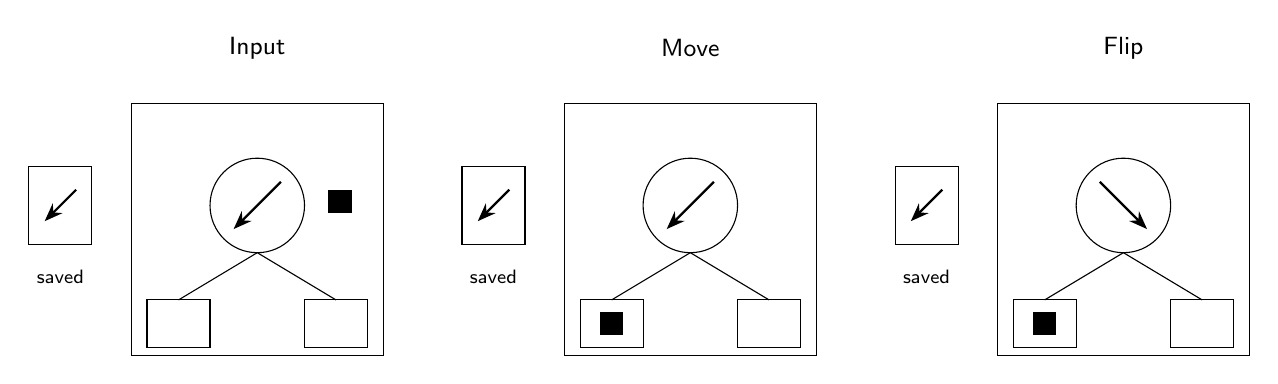
\begin{tikzpicture}[x=1mm,y=1mm,>=Stealth,font=\small]
\foreach \x/\label/\state in {0/Input/0,55/Move/1,110/Flip/2}{
  \begin{scope}[shift={(\x,0)}]
    \node at (0,20) {\label};
    \draw (-16,13) rectangle (16,-19);
    \draw (0,0) circle (6);
    \draw (0,-6)--(-10,-12) (0,-6)--(10,-12);
    \draw (-14,-12) rectangle (-6,-18) (6,-12) rectangle (14,-18);
    \draw (-29,-5) rectangle (-21,5);
    \draw[->,thick] (-23,2)--(-27,-2);
    \node[font=\scriptsize] at (-25,-9) {saved};
    \ifnum\state<2 \draw[->,thick] (3,3)--(-3,-3);
    \else \draw[->,thick] (-3,3)--(3,-3);\fi
    \ifnum\state=0 \fill (9,-1) rectangle (12,2);
    \else \fill (-11.5,-16.5) rectangle (-8.5,-13.5);\fi
  \end{scope}}
\end{tikzpicture}
\end{center}
The black square is the counter. The saved arrow does not change. With blank exits there is no letter to record yet; once X and Y are named, one arrival fills one box. The adult can point to the next box and write the child's named letter. On the tree, keep the three saved cards in a matching top/left/right arrangement \emph{off} the board. Copy from these, never from changed working cards. Keep later arrivals waiting while recording catches up.

\textbf{A one-hour first route.} Allow 5 minutes for movement, 5 for the shared launch, 3 for table setup, 15 for Problems 1--2, 10 for Problem 3, and 15 for Problem 5 if partners manage flips independently; reserve 7 for sharing and packing. These are adjustable estimates, not a completion schedule. Stop with the switch if it still needs practice. Save Problem 4's prediction game and Problems 6--9 for another visit, or offer one to a ready pair. One careful contrasting trial can be enough; not every recording row must be filled.

\sub{Problem 1, student page 1: ten arrivals}
From first arrow X: \code{XYXYXYXYXY}. From Y: \code{YXYXYXYXYX}. Neither has two consecutive arrivals at the same exit; each leaves five at each exit. A child may point to the flipped arrow as the reason the next arrival must change. Ask only if needed: ``Where is the arrow pointing now?'' or ``Could that same exit be next without changing a rule?'' Later ask whether any exit can ever be two ahead.

\sub{Problem 2, student page 2: all six pile pictures}
Read pictures left to right, top row then bottom row. X is left, Y is right.
\begin{center}
\begin{tabular}{ccccccc}
\toprule
Picture & 1 & 2 & 3 & 4 & 5 & 6\\
\midrule
Piles X,Y & 2,1 & 3,3 & 2,3 & 5,2 & 5,4 & 3,5\\
Start & X & either & Y & impossible & X & impossible\\
\bottomrule
\end{tabular}
\end{center}
The two starts exhaust the choices. Pair arrivals: each pair supplies one to each exit, with at most one unpaired counter going to the first arrow's exit. This rules out pictures 4 and 6. Use the saved card when drawing the start: after an odd number of counters the working card points the other way. Hint: ``Can you match each X counter with a Y counter? How many are left unmatched?''
\newpage

\head{Coins, predictions and the four-exit tree}
\sub{Problem 3, student page 3: a coin can repeat}
Both answers are yes. Agree aloud that heads means X and tails Y, then put the switch card away. For example, the possible toss order heads, heads, heads, heads, heads, tails, tails makes \code{XXXXXYY}: two consecutive counters share an exit, and the piles are five and two. A child may invent any other witness. A proposed sequence is not a claim that those tosses actually occurred.

There are six seven-box rows, not a requirement to keep tossing until a success. For fair independent tosses, 42 of the 128 seven-toss orders give five and two in either direction. Even six trials miss that split about 9.2\% of the time. If it never appears, ask ``What faces would make the piles? Could the coin show those faces?'' A short run cannot establish impossibility or that a coin must balance. Keep the counts as adult background; children need only the possible face-by-face story.

\sub{Problem 4, student page 3: predict before continuing}
The printed table lists counters 5, 8, 7 and 4 in that order. After watching counter 1, make \emph{all four guesses first}. Continue the same trial through counter 8, without resets; the adult fills ``landed'' when counter 4, then 5, then 7, then 8 arrives. Thus the out-of-order rows do not require going backwards or separate trials. Keep a single arrival strip if needed.
\begin{center}
\begin{tabular}{ccccc}
\toprule
Counter & 5 & 8 & 7 & 4\\
\midrule
Card, compared with counter 1 & same & other & same & other\\
\bottomrule
\end{tabular}
\end{center}
If counter 1 was X, the four predictions are X, Y, X, Y; if Y, they are Y, X, Y, X. The arrow alternates at every departure, so returning in pairs explains the pattern. For the coin there is no guaranteed prediction: either exit is possible at each listed counter, regardless of the first toss. Under the fair independent model each guess has probability one half, not certainty. Hint: ``What does the card remember that the coin does not?'' Correct guesses alone do not make the coin predictable.

\sub{Problem 5, student page 4: can two of four share an exit?}
No, from any start. Two go to each lower card, and each lower card sends its two to different exits. Let children show that with the four counters before giving the full argument. Ask ``How many reached each lower card? What did that card do with its two?''

For adult lookup, L means down-left and R down-right. A three-letter word lists \textbf{top, left lower, right lower} cards, not exit letters. Use physical saved cards with children instead. The complete list is:
\begin{center}
\begin{tabular}{cc@{\hspace{20mm}}cc}
\toprule
Start & First four arrivals & Start & First four arrivals\\
\midrule
\code{LLL} & \code{ACBD} & \code{RLL} & \code{CADB}\\
\code{LLR} & \code{ADBC} & \code{RLR} & \code{DACB}\\
\code{LRL} & \code{BCAD} & \code{RRL} & \code{CBDA}\\
\code{LRR} & \code{BDAC} & \code{RRR} & \code{DBCA}\\
\bottomrule
\end{tabular}
\end{center}
Each of three cards has two choices, giving $2\times2\times2=8$ starts. The student page has nine recording trees: one is spare, not evidence for a ninth start. If the children want a complete check, pool distinct starts across pairs and use this page's saved drawings again for Problem 6; do not require every child to repeat all eight. Four counters also return every card to its start, so counters 5--8 repeat the order. A natural continuation is to predict the next four before sending them.
\newpage

\head{Pile targets and programming the start}
All card words below use top, left lower, right lower order, as defined on guide p.\ 3. A list gives \emph{every} successful start, though most problems ask for just one. Keep the saved cards visible throughout each trial.

\sub{Problem 6, student page 5: six pile pictures}
Read each row left to right, then move down. Piles are in A, B, C, D order.
\begin{center}
\begin{tabular}{cccl}
\toprule
Picture & Counters & Piles & All successful starts\\
\midrule
1 (top left) & 8 & 2,2,2,2 & all eight\\
2 (top right) & 6 & 2,1,2,1 & \code{LLL}, \code{RLL}\\
3 (middle left) & 6 & 2,2,1,1 & impossible\\
4 (middle right) & 12 & 3,3,3,3 & all eight\\
5 (bottom left) & 6 & 1,2,1,2 & \code{LRR}, \code{RRR}\\
6 (bottom right) & 8 & 3,1,2,2 & impossible\\
\bottomrule
\end{tabular}
\end{center}
Four-counter blocks give one to each exit, so pictures 1 and 4 always work and picture 6 never does. After six, the top card has sent three to each side; picture 3 wants four left and two right. For picture 2 the lower cards must first favor A and C; for picture 5, B and D; either top direction works. These reasons cover every start, as does the complete eight-start list. Hint: ``How many counters would this picture need on each side of the top card?'' Have children copy saved arrows, not the lower cards that have just flipped three times.

\sub{Problem 7, student page 6: B first or last to get two}
B is first to two at counter 5 from \code{LRL} or \code{LRR}; their orders begin \code{BCAD} or \code{BDAC}. B is last to two at counter 8 from \code{RLL} or \code{RLR}; their orders begin \code{CADB} or \code{DACB}. No exit gets a second until each has one, and the next round repeats the first. Thus B must be first or last in that first round. Hint: ``When the next round starts, which exit will be visited first?'' The start list proves these are all the choices. Draw from the saved cards before testing, even if stopping as soon as B gets two.

\sub{Problem 8, student page 6: every start with C first}
Exactly two complete settings: \code{RLL} and \code{RRL}. The top card must send the counter right; the right lower card must send it left to C. The left lower card is never touched, so either direction works. ``The left card doesn't matter'' is the structural answer; accept that insight, then show its two settings. The third printed tree is spare space, not a missing third answer. Hint: ``Which card did your counter never visit?'' Once ready, children can choose a different first exit and ask which card becomes free.

\sub{Problem 9, student page 7: the first two exits}
Top left, A then D: \code{LLR} only. Top right, D then C: impossible. Bottom left, C then B: \code{RRL} only. Bottom right, B then A: impossible. The first two counters must go to opposite sides of the top card; C and D share one side, as do A and B. In a possible picture, the first counter fixes the top and one lower card; the second fixes the other lower card, so no choice is left. Hint: ``Where must counter 2 go when the top card has flipped?''

\textbf{Where it goes.} Once the pages are approved, this section replaces ``K--1 route, adult-read'' under ``Preparation, launch and visit choices'' on page 2 of \code{week-91-facilitator.pdf} (F91-FAC-v3), including its final two lines at the top of page 3. It does not replace the shared launch or older-band solutions.
\end{document}
